\chapter{Overview}\label{s:overview}
This overview contains a Utility Tree, which captures the Architecturally Significant Requirements (ASR). These ASRs are extracted from interviews (interviewee description in Appendix  \ref{Appendix A}) and combined with the Business Goals and Concerns (available in Appendix \ref{Appendix B} and  \ref{Appendix C}) 
% Tabel laten beginnen met kolom ASR. Dit bepaald immers de volgorde van de regels uit de tabel. Of de volgorde laten afhangen van BG nummering

\begin{table}[h!]
\centering
\begin{tabular}{||l l l||} 
 \hline
 Business Goal(s) (BG) & Concern(s) (C) & Architecturally Significant Requirement (ASR) \\ [0.5ex] 
 \hline\hline
 \makecell {BG-03} & C-03 & ASR-1 Confidentiality \\
 \hline
 \makecell {BG-01, BG-02} & C-01, C-02 & ASR-2 Re-usability\\
\hline
 \makecell {BG-05} &  C-09 & ASR-3 Maturity  \\
 \hline
\makecell {BG-04} & C-04, C-05, C-06, C-11 & ASR-4 Authenticity \\
 \hline
 \makecell {BG-01} & C-10 & ASR-5 Accountability  \\ [1ex] 
 \hline
\end{tabular}
\caption{ASRs Plotted on business goals and concerns.}
\label{ASR_BG_C}
\end{table}

Concerns C-07, C-08 and \todo{C-11} and BG-06 are not addressed in this overview because the scope of this research is not taking into account possible required changes in law and processes within non-government organizations. However, these concerns are considered possibly relevant for future research and therefore included in the appendix.

 \begin{longtable}[c]{|p{4cm}|p{8cm}|p{2cm}|}
 \caption{Example of a Business Goal. Complete list available in Appendix \ref{Appendix B} Table \ref{tab:business_goals}\label{tab:Example_business_goals}}\\
 \hline
 \multicolumn{3}{| c |}{Begin of Table}\\
 \hline
 Business Goal number and name & Description & Addressed by\\
 \hline
 \endfirsthead

 \hline
 \multicolumn{3}{|c|}{Continuation of Table \ref{tab:business_goals}}\\
 \hline
 Business Goal number and name & Description & Addressed by\\
 \hline
 \endhead

 \hline
 \endfoot

 \hline
 \multicolumn{3}{| c |}{End of Table}\\
 \hline\hline
 \endlastfoot
 BG-01 Explainable solutions   &   Communicate in a simple manner how technology works to raise awareness and support. Also, provide more detailed scientific information for experts to contribute as a community. &  I-03\\
 \end{longtable}
 
 \begin{longtable}[c]{|p{4cm}|p{8cm}|p{2cm}|}
 \caption{Example of a Concern. Complete list available in Appendix \ref{Appendix C} Table \ref{tab:concerns}\label{tab:Example_concerns}}\\
 \hline
 \multicolumn{3}{| c |}{Begin of Table}\\
 \hline
 Concern number and name & Description & Addressed by\\
 \hline
 \endfirsthead

 \hline
 \multicolumn{3}{|c|}{Continuation of Table \ref{tab:business_goals}}\\
 \hline
 Concern number and name & Description & Addressed by\\
 \hline
 \endhead

 \hline
 \endfoot

 \hline
 \multicolumn{3}{| c |}{End of Table}\\
 \hline\hline
 \endlastfoot
 C-01 Knowledge of systems and what is legally allowed    &   Area of expertise within the identity domain is complex and system specialists (NL: Stelselspecialisten) and other specialists are a rare resource. History of law and systems is implicit knowledge or hard to find in documentation. When designing new systems it's needed to comprehend the domain and its internal and external influences. & I-03\\
 \end{longtable}


    
    \begin{figure}
        \graphicspath{ {./images/} }
        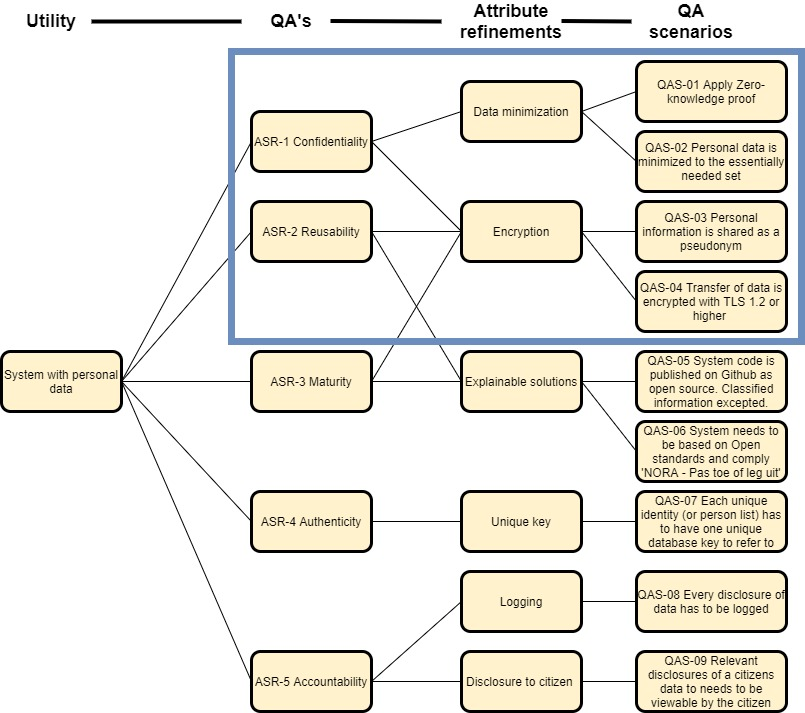
\includegraphics[width=17cm]{Decomposition of ASR and QAS-Utility Tree v3.jpg}\\
        \caption{Decomposition of Architecturally significant requirements}
        \label{fig:ASR1}
    \end{figure}
    % Vragen over het figuur - puur inhoudelijk - negeer vooral als je geen izn hebt: in 1.3 staat het volgende "Thereafter, combining these goals and concerns in a formal description of ArchitecturallySignificant Requirements (ASR) categorized in Quality attributes (QA)". Hieruit haal ik daat Quality Attributes een groepering is van ASR's. Maar in de figuur lijken ze synoniemen. Daarnaast zie ik in de figuur een attribute refinement staan die "Explainable solutions" heet. Dit is gelijk aan de naam van BG-1. Vallen Business goals (en wellicht ook concerns), onder de noemer Attribute refinement? Of is dit puur toeval. Als lezer mis ik misschien een stukje relaties tussen QA's, ASRs, BGs en Cs.